\documentclass{beamer}

% Theme choice
\usetheme{Madrid}

% Optional packages
\usepackage{graphicx} % For including images
\usepackage{amsmath}  % For math symbols and formulas
\usepackage{hyperref} % For hyperlinks

% Small helpers for simple boxes in diagrams
\newcommand{\ovbox}[2]{\colorbox{#1}{\strut\parbox[c][1.2em]{0.6\linewidth}{\centering #2}}}
\newcommand{\ovpbox}[2]{\colorbox{#1}{\strut\parbox[c][1.2em]{0.15\linewidth}{\centering #2}}}
\setlength{\fboxsep}{6pt}

% Where to look for images (put the OpenVINO logo into one of these)
\graphicspath{{./assets/}{./images/}}

\title[OpenVINO introduction]{OpenVINO introduction}
\author{Obolenskiy Arseniy, Nesterov Alexander}
\institute{ITLab}

\date{\today}

% Redefine the footline to display both the short title and the org name
\setbeamertemplate{footline}{
  \leavevmode%
  \hbox{%
    \begin{beamercolorbox}[wd=.45\paperwidth,ht=2.5ex,dp=1ex,leftskip=1em,center]{author in head/foot}%
        \usebeamerfont{author in head/foot}\insertshortinstitute% Displays the university name
    \end{beamercolorbox}%
    \begin{beamercolorbox}[wd=.45\paperwidth,ht=2.5ex,dp=1ex,leftskip=1em,center]{author in head/foot}%
      \usebeamerfont{author in head/foot}\insertshorttitle% Displays the short title
    \end{beamercolorbox}%
    \begin{beamercolorbox}[wd=.1\paperwidth,ht=2.5ex,dp=1ex,rightskip=1em,center]{author in head/foot}%
      \usebeamerfont{author in head/foot}\insertframenumber{} / \inserttotalframenumber%
    \end{beamercolorbox}}%
  \vskip0pt%
}

\AtBeginSection[]{
  \begin{frame}
    \centering
    \Huge\insertsection%
  \end{frame}
}

\begin{document}

\begin{frame}
  \titlepage%
\end{frame}

\begin{frame}{Contents}
  \tableofcontents
\end{frame}

\section{Overview}
\begin{frame}{What is OpenVINO?}
  \begin{columns}[T,totalwidth=\textwidth]
    \begin{column}{0.7\textwidth}
      OpenVINO (Open Visual Inference and Neural Network Optimization)
      is a toolkit developed by Intel for optimizing and deploying deep learning models
      for inference on Intel hardware. It provides a unified API and a set of tools to streamline
      the process of model optimization, conversion, and deployment across various Intel architectures.
    \end{column}
    \begin{column}{0.25\textwidth}
      \centering
      
\includegraphics[width=\linewidth]{openvino-logo.png}
    \end{column}
  \end{columns}
\end{frame}

\begin{frame}{OpenVINO at a Glance}
  \begin{itemize}
    \item \textbf{Purpose:} Optimize and deploy AI inference across Intel CPUs, GPUs, NPUs, and other accelerators
    \item \textbf{Core components:} Model Optimizer, Runtime (Inference Engine), Post-Training Optimization Tool, Benchmark tools, Notebooks
    \item \textbf{Model formats (Frontends):} IR (\texttt{.xml/.bin}), ONNX (\texttt{.onnx}), TensorFlow (SavedModel/MetaGraph/frozen \texttt{.pb/.pbtxt}), TensorFlow Lite (\texttt{.tflite}), PaddlePaddle (\texttt{.pdmodel}), PyTorch (TorchScript/FX)
    \item \textbf{Targets:} CPU, iGPU, dGPU (e.g., Intel Arc), NPU, and more via plugins
    \item \textbf{Key benefits:} Performance, portability, unified API, quantization (INT8), easy deployment
  \end{itemize}
  \footnotesize Reference: \href{https://docs.openvino.ai/}{docs.openvino.ai}
\end{frame}

\begin{frame}{Overview Diagram}
  \centering
  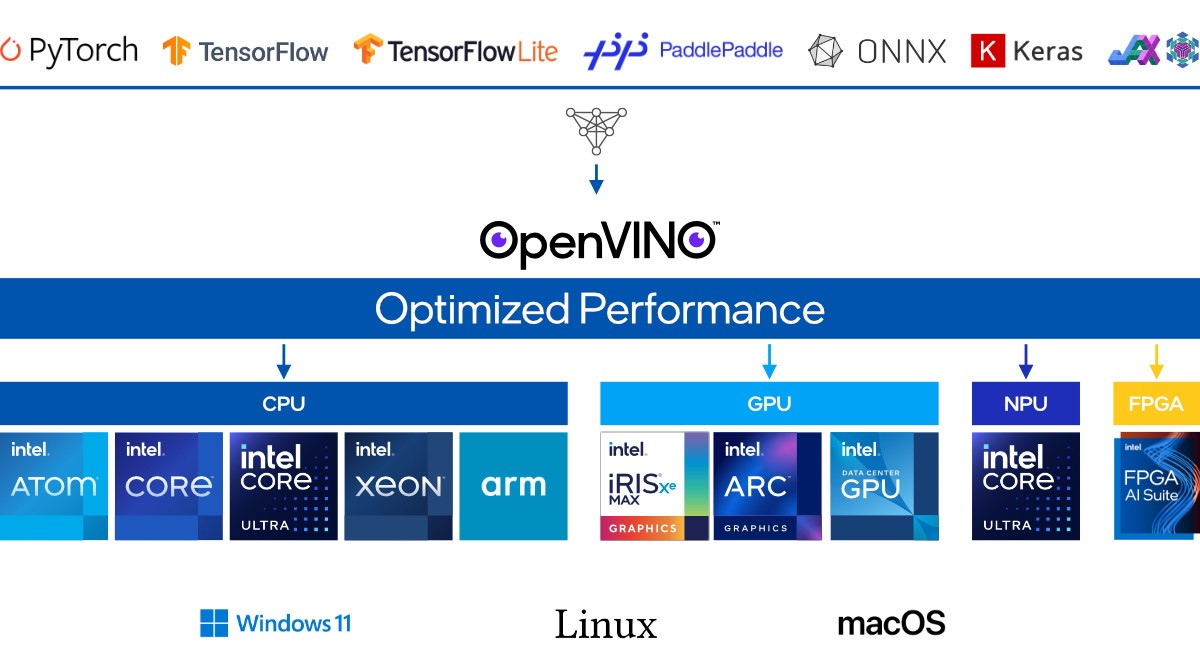
\includegraphics[width=\textwidth]{openvino-overview-diagram.jpg}
  \footnotesize Source: \href{https://docs.openvino.ai/2025/_images/openvino-overview-diagram.jpg}{https://docs.openvino.ai/2025/index.html}
\end{frame}

\begin{frame}{Workflow Overview}
  \centering
  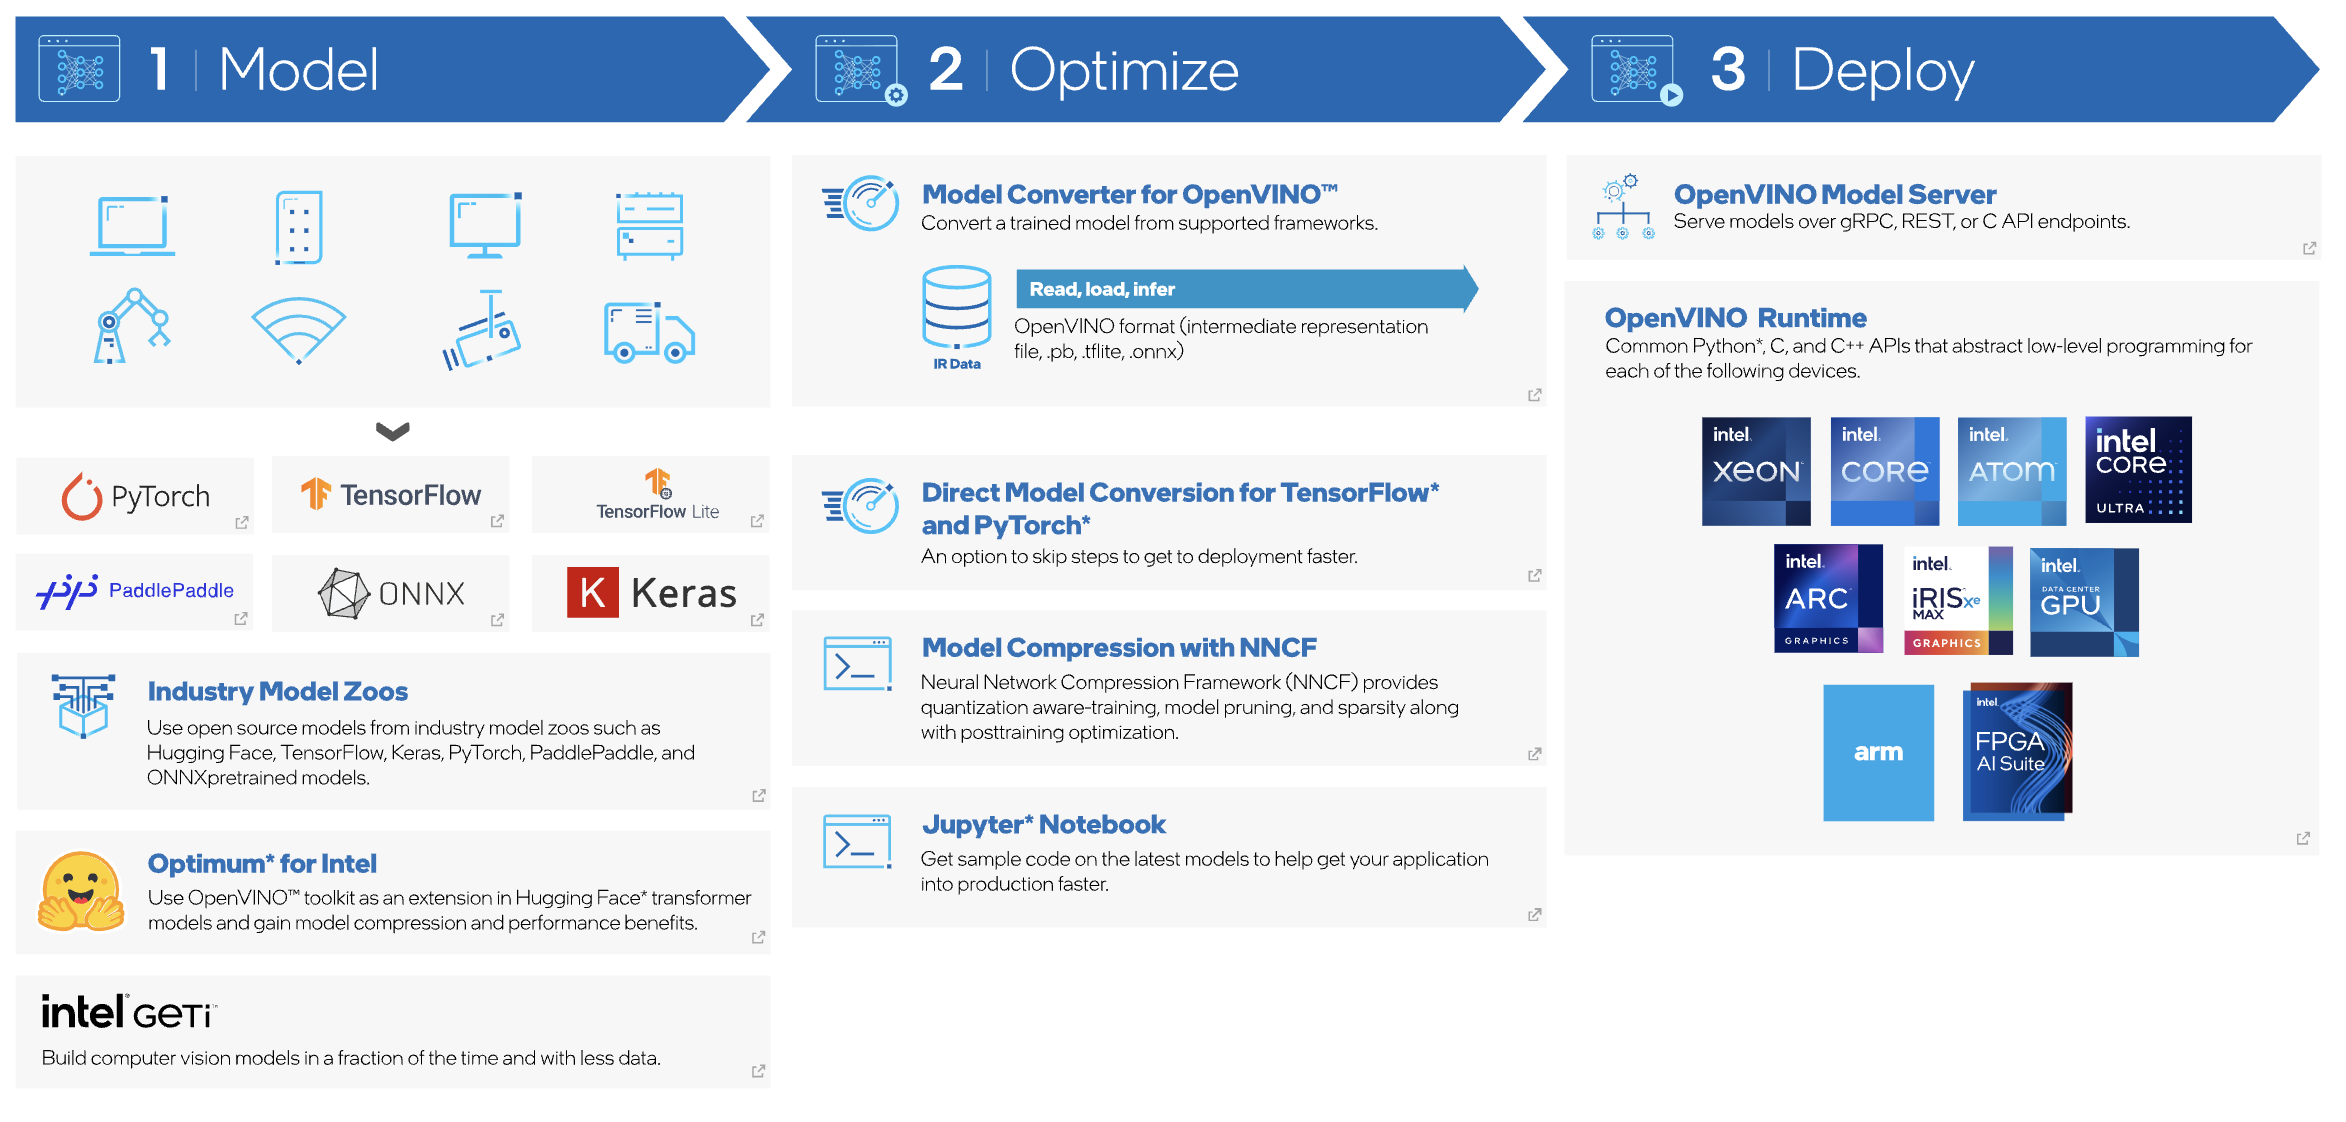
\includegraphics[width=\textwidth]{openvino-use-case.png}
  \footnotesize Source: \href{https://www.intel.com/content/www/us/en/developer/tools/openvino-toolkit/overview.html}{https://www.intel.com/content/www/us/en/developer/tools/openvino-toolkit/overview.html}
\end{frame}

\begin{frame}{Device Plugins Architecture}
  \centering
  \ovbox{gray!15}{\textbf{Application} (C++/Python)}\\[0.6em]
  $\Downarrow$\\[0.2em]
  \ovbox{gray!15}{\textbf{OpenVINO Runtime} (\texttt{ov::Core})}\\[0.6em]
  $\Downarrow$\\[0.2em]
  \ovbox{blue!10}{\textbf{Plugin Dispatcher} (AUTO / MULTI / HETERO)}\\[0.8em]
  $\Downarrow$\\[0.6em]

  % Row of device plugins
  \ovpbox{gray!20}{CPU}\hspace{0.6em}%
  \ovpbox{green!15}{GPU}\hspace{0.6em}%
  \ovpbox{magenta!15}{NPU}%

  \vspace{0.6em}
  \footnotesize Examples: \texttt{CPU}, \texttt{GPU.0}, \texttt{NPU}, \texttt{AUTO:CPU,GPU}, \texttt{MULTI:GPU,CPU}, \texttt{HETERO:GPU,CPU}
\end{frame}

\begin{frame}{Device Plugin Details}
  \begin{itemize}
    \item \textbf{CPU}: High compatibility and strong baseline performance; uses optimized kernels (e.g., oneDNN). Supports FP32/FP16/INT8 with quantized models.
    \item \textbf{GPU}: Integrated and discrete Intel GPUs via Level Zero/OpenCL, delivering strong FP16 and INT8 throughput and benefiting from device-specific kernels and memory bandwidth.
    \item \textbf{NPU}: Intel NPU (e.g., Core Ultra) for efficient, low-power inference on common vision/LLM ops; ideal for always-on and battery-sensitive workloads.
    \item \textbf{TEMPLATE plugin}: Reference backend for building custom device plugins; demonstrates the plugin API (compiled model, infer request, op support, memory) and is useful for prototyping.
  \end{itemize}
  \footnotesize See: \href{https://docs.openvino.ai/2025/documentation/compatibility-and-support/supported-devices.html}{https://docs.openvino.ai/2025/documentation/compatibility-and-support/supported-devices.html} \;\;|\;\; \href{https://docs.openvino.ai/2024/openvino_docs_OV_UG_supported_plugins_Supported_Devices.html}{Supported devices}
\end{frame}

\begin{frame}{Inference Modes}
  \begin{itemize}
    \item \textbf{AUTO plugin}: Chooses the “best” device available at runtime; can constrain candidates, e.g., \texttt{AUTO:GPU,CPU}.
    \item \textbf{MULTI plugin}: Executes across multiple devices in parallel to maximize throughput, e.g., \texttt{MULTI:GPU,CPU}.
    \item \textbf{HETERO plugin}: Splits a single graph by layer/op support across devices, e.g., heavy ops on GPU, fallbacks on CPU\@.
  \end{itemize}
  \footnotesize See: \href{https://docs.openvino.ai/2025/openvino-workflow/running-inference/inference-devices-and-modes.html}{https://docs.openvino.ai/2025/openvino-workflow/running-inference/inference-devices-and-modes.html} \;\;|\;\; \href{https://docs.openvino.ai/2024/openvino_docs_OV_UG_supported_plugins_Supported_Devices.html}{Inference Devices and Modes}
\end{frame}

\section{References}
\begin{frame}{References}
  \begin{itemize}
    \item OpenVINO Official documentation: \href{https://docs.openvino.ai/}{https://docs.openvino.ai/}
    \item OpenVINO repository: \href{https://github.com/openvinotoolkit/openvino}{https://github.com/openvinotoolkit/openvino}
    \item OpenVINO Contrib: \href{https://github.com/openvinotoolkit/openvino_contrib}{https://github.com/openvinotoolkit/openvino\_contrib}
    \item OpenVINO Notebooks: \href{https://github.com/openvinotoolkit/openvino_notebooks}{https://github.com/openvinotoolkit/openvino\_notebooks}
  \end{itemize}
\end{frame}

\end{document}
